\lstset{language=Java, numbers=left, numberstyle=\tiny, stepnumber=2, numbersep=5pt}
\chapter{Introduction}
\label{intro}
The aim of this workshop was to gain first experiences about intelligent systems in a real world. The task was based on a thermal model of a house simulated by Simulink\footnote{https://de.mathworks.com/products/simulink.html}, a graphical interface of MATLAB\footnote{https://de.mathworks.com/products/matlab.html}.
The model provided had to be understood and, if possible, improved with regard to a constant temperature in the house and low heating costs.
\\
The first main task was to modify the model so that it could be used to generate data for the training.
This training data should be used to develop an Artificial Neural Network (ANN) model of
the house. The resulting model should be tested and compared with the original house model.
\\
The second task is to provide a fuzzy logic controller for the temperature control of the
house in relation to the temperature outside the house, which should replace the binary logic of the existing thermostat.

%%%%%%%%%%%%%%%%%%%%%%%%%%%%%%%%%%%%%%%%%%%%%%%%%%%%%%%%%%%%%%%%%%%%%%%%%%%%%%%%%%%%%%%%%%%%%%%%%%%%%%%%%
%%%%%%%%%%%%%%%%%%%%%%%%%%%%%%%%%%%%%%%%%%%%%%%%%%%%%%%%%%%%%%%%%%%%%%%%%%%%%%%%%%%%%%%%%%%%%%%%%%%%%%%%%
%%%%%%%%%%%%%%%%%%%%%%%%%%%%%%%%%%%%%%%%%%%%%%%%%%%%%%%%%%%%%%%%%%%%%%%%%%%%%%%%%%%%%%%%%%%%%%%%%%%%%%%%%
\chapter{Neural Network}
\label{neuralnetwork}
An artificial neural network is a network of artificial neurons that mimic the functioning of a living organism's brain and thus are capable of machine learning with training data \cite[][]{DK01}. The aim of this first part of the workshop was to improve an existing model of a house with a central, intelligent heating system, using an ANN, which is to be trained using data from the existing heating system.
\section{Thermal model}
The house's existing thermal model has complex logic implemented in Simulink using logic blocks. The model is able to realistically depict the temperature fluctuations that the house undergoes during the course of a day in comparison with the outside temperature. 
\section{Generating training data}
Now the model was used to collect training data for the new Artificial Neural Network. For this the model had to be easily adapted to save the generated data in the Matlab workspace. For this to succeed, the parameters that the model of the house needs to calculate its output data must first be understood. The house model has two input and one output parameter:
\begin{itemize}
	\item \textbf{Input:} Temperature Error (desired room temperature - actual indoor temperature value)
	\item \textbf{Input:} Outdoor temperature
	\item \textbf{Output:} new room temperature
\end{itemize}
To store the output values in the workspace, a multiplexer was used, which passes the values for the outdoor temperature, the error and the resulting internal temperature to a simout block. This block stores the data in the workspace. Figure \ref{housesetup} shows the modified Simulink Model of the House:
\begin{figure}[H]
	\centering
	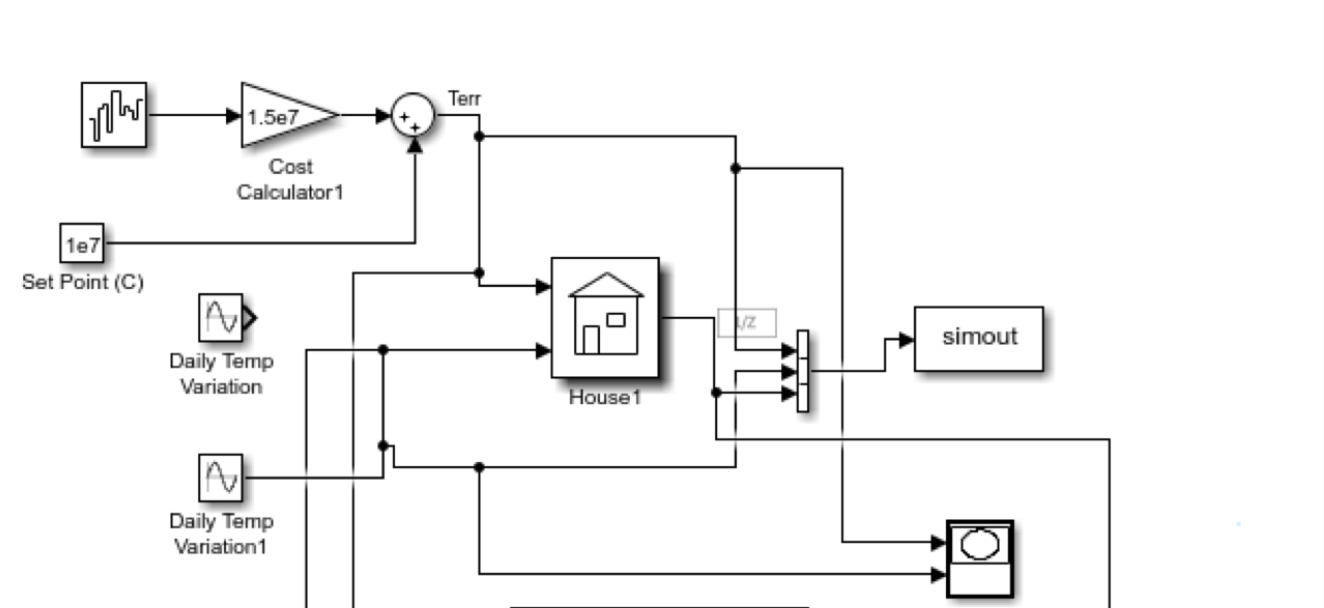
\includegraphics[width=1.0\linewidth]{1housesetup.png}
	\caption[Caption for LOF]{Simulink model modified for generating training data.}
	\label{housesetup}
\end{figure}
\section{Configuration and Training}
The next step was to use Matlab to design an ANN that would be trained using the previously saved values of the original house model. Matlab offers a tool that allows the user to design a Simulink block for his own ANN. The only difficulty here is to configure the number of hidden layers and the number of respective neurons in each hidden layer so that the ANN comes as close as possible to the desired output data for the internal temperature using the input data provided. Figure \ref{neural} shows the Design for the ANN in Matlab as well as the number of Hidden Layers an Neurons:
\begin{figure}[H]
	\centering
	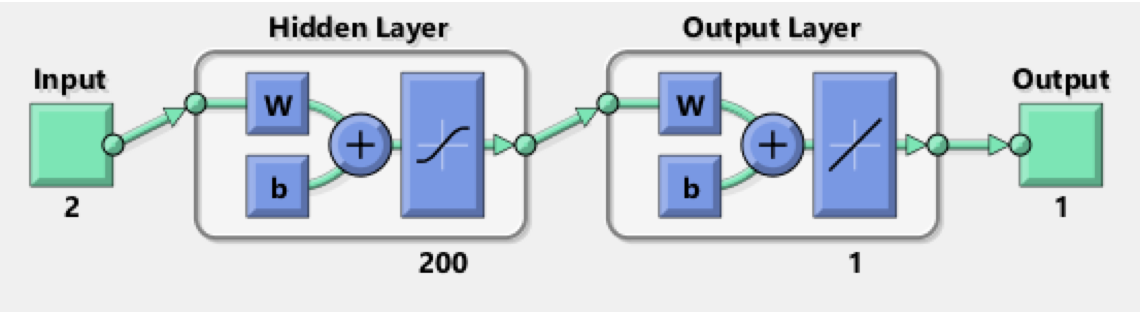
\includegraphics[width=1.0\linewidth]{1neural.png}
	\caption[Caption for LOF]{Neural network configuration.}
	\label{neural}
\end{figure}
After several attempts it was found that 200 neurons in a hidden layer are sufficient to achieve a satisfactory approximation of the ANN to the original house model. The deviation of the results between the ANN and the house model was only 0.2 percent, which is a very good result. Figure \ref{training} shows the results for the configured ANN and the match \textbf{R} between the results of the ANN and the output data collected from the training data set of the house model.
\begin{figure}[H]
	\centering
	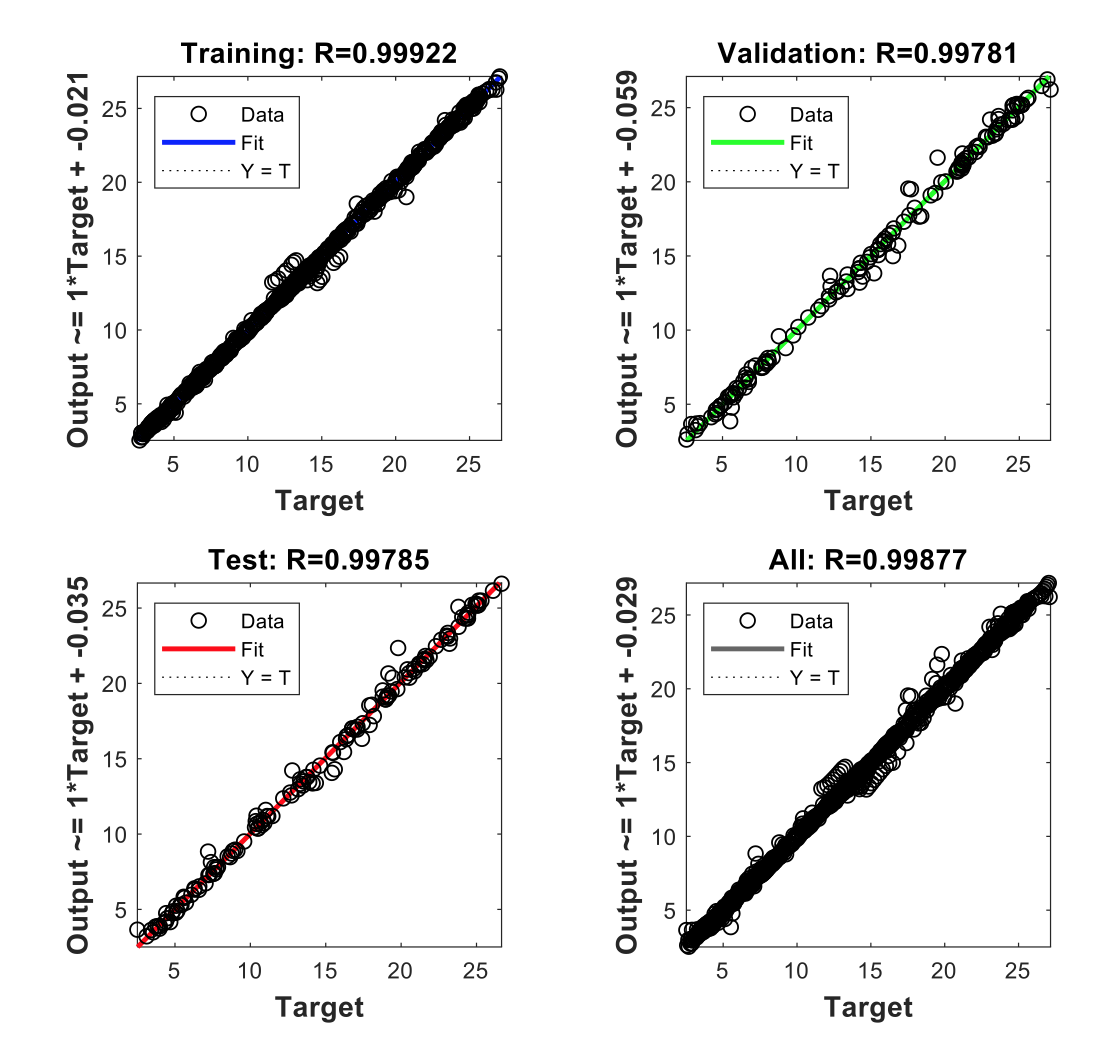
\includegraphics[width=1.0\linewidth]{1trainingresult.png}
	\caption[Caption for LOF]{Training results}
	\label{training}
\end{figure}
\section{Analysis and Evaluation}
In the last step of this first task, the Simulink model was modified to allow comparison of the two models. The Simulink block of the ANN is inserted into the original Simulink model and receives the same inputs as the house model. The outputs of both blocks are then plotted and compared. Figure \ref{houseneural} shows this modified Version of the original Model:
\begin{figure}[H]
	\centering
	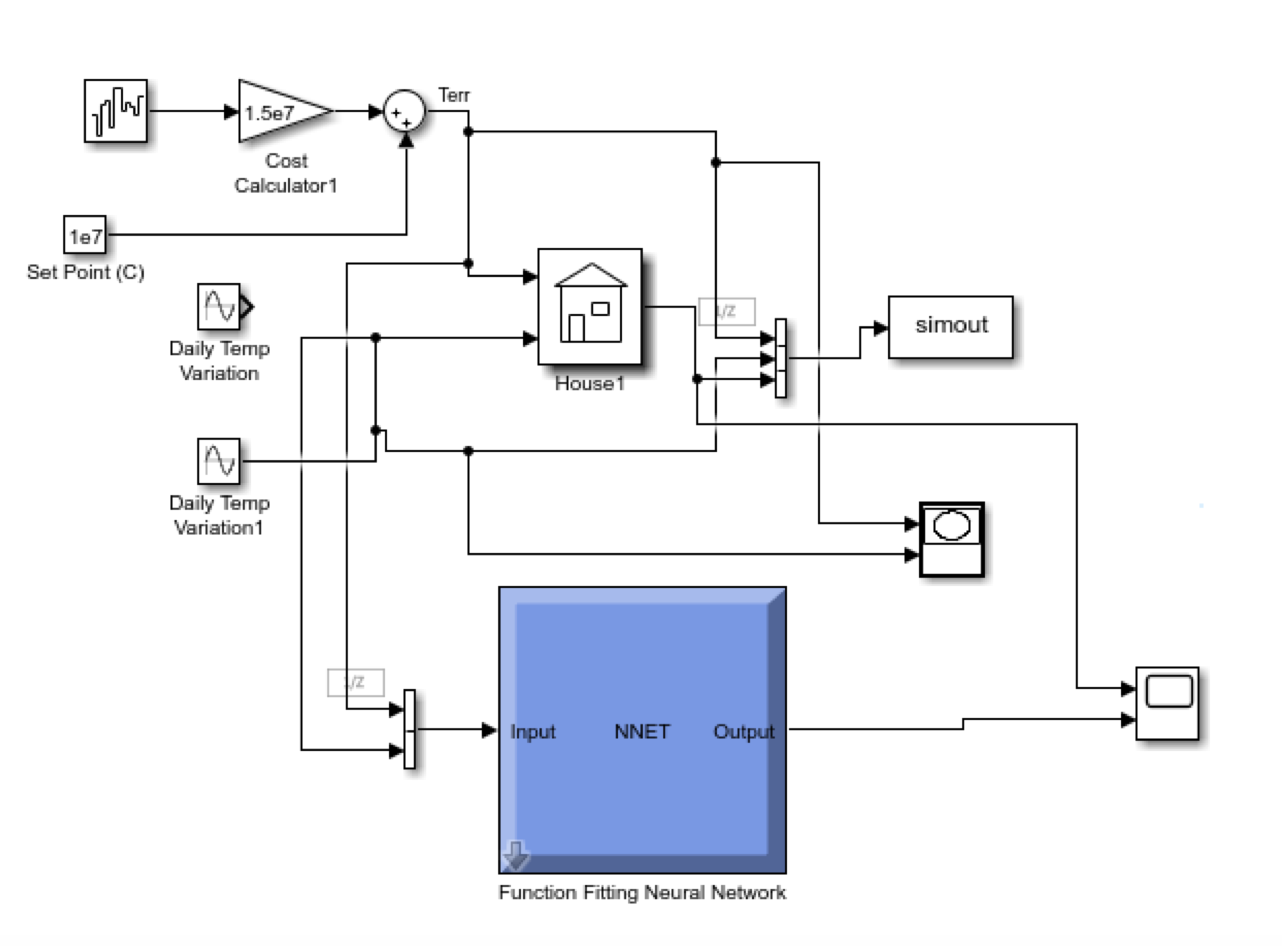
\includegraphics[width=1.0\linewidth]{1houseneural.png}
	\caption[Caption for LOF]{The original Simulink model modified using the neural network}
	\label{houseneural}
\end{figure}
Figure \ref{origvsneural} shows the comparison between the outputs of the House Model and the neural network:
\begin{figure}[H]
	\centering
	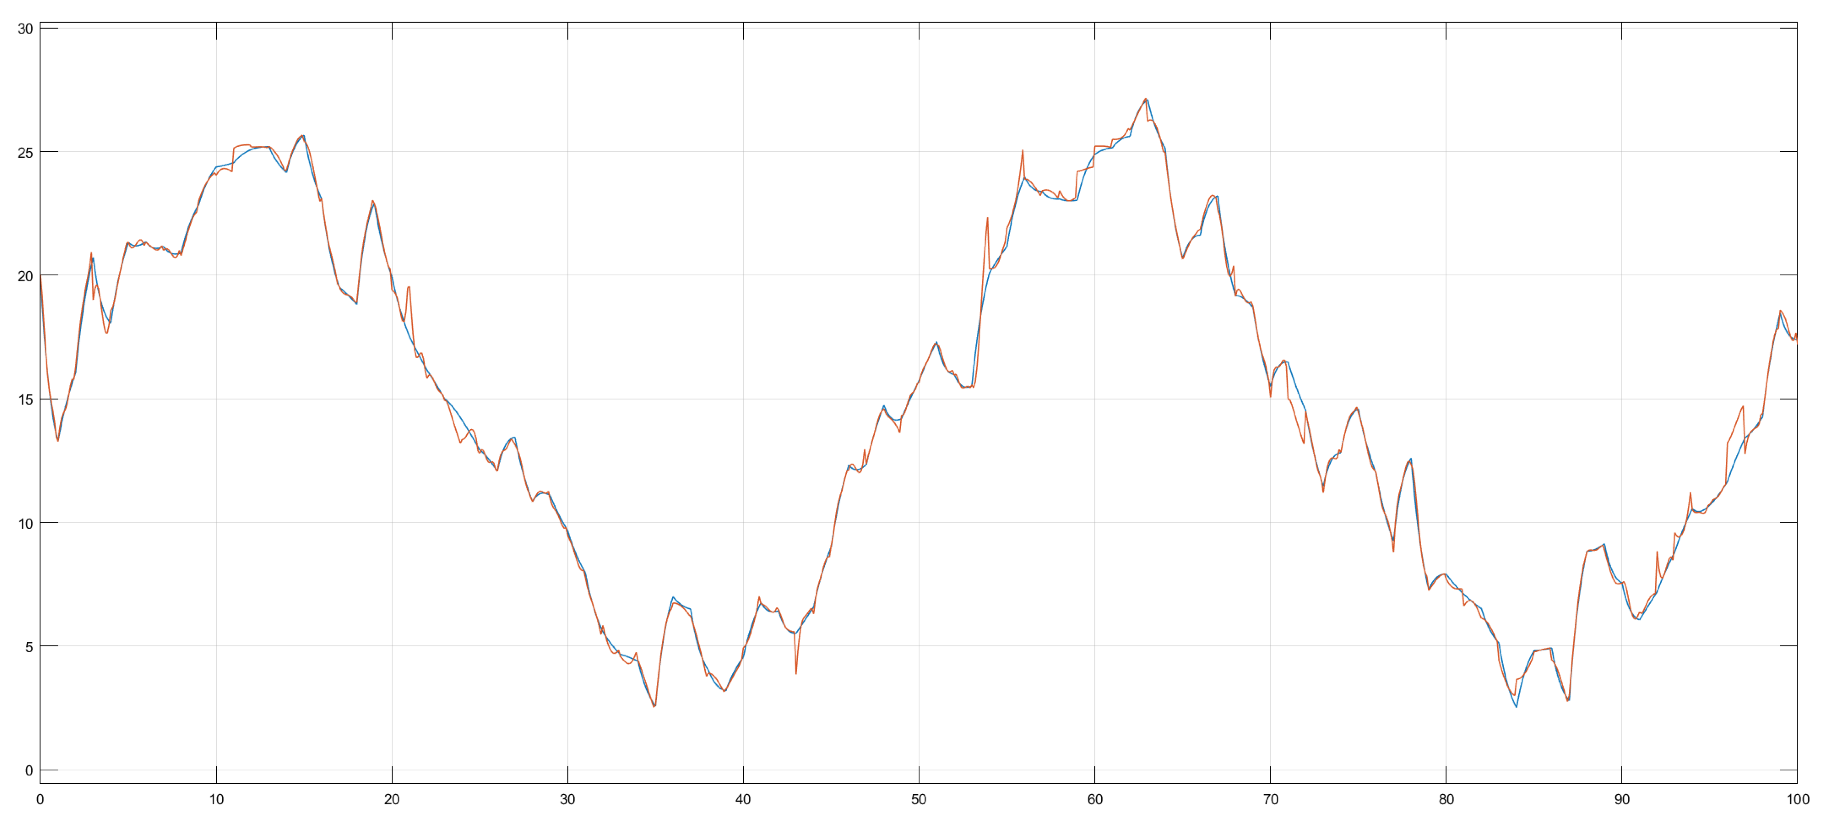
\includegraphics[width=1.0\linewidth]{1origvsneural.png}
	\caption[Caption for LOF]{Original house simulation (blue), trained neural network (red)}
	\label{origvsneural}
\end{figure}
It can be seen that the curves are very close to each other with single small escapees here and there. But all in all it can be said that the ANN can almost perfectly take over the function of the house model without major fluctuations in the output values being noticeable. This shows how easily a neural network can perform the function of complex logic for a problem in the real world. All it takes is a set of useful training data.
%%%%%%%%%%%%%%%%%%%%%%%%%%%%%%%%%%%%%%%%%%%%%%%%%%%%%%%%%%%%%%%%%%%%%%%%%%%%%%%%%%%%%%%%%%%%%%%%%%%%%%%%%
%%%%%%%%%%%%%%%%%%%%%%%%%%%%%%%%%%%%%%%%%%%%%%%%%%%%%%%%%%%%%%%%%%%%%%%%%%%%%%%%%%%%%%%%%%%%%%%%%%%%%%%%%
%%%%%%%%%%%%%%%%%%%%%%%%%%%%%%%%%%%%%%%%%%%%%%%%%%%%%%%%%%%%%%%%%%%%%%%%%%%%%%%%%%%%%%%%%%%%%%%%%%%%%%%%%
\chapter{Fuzzy Logic}
\label{fuzzy}
A big problem for developers of intelligent systems is to teach a computer in some way that for decisions in complex situations it is not sufficient to calculate two or more possibilities that are strictly separated from each other. A computer should be able to analyze more complex situations and make decisions like a human being that classify output data into several categories that are not necessarily clearly separated. \cite[][]{LB01}
\section{The original setup and problem}
\label{problem}
In this real example, the system uses a thermostat that regulates the inside temperature of the house according to the outside temperature and the difference between the outside and inside temperature. Figure \ref{housetermo} shows the original setup of the Simulink Model with the thermostat:
\begin{figure}[H]
	\centering
	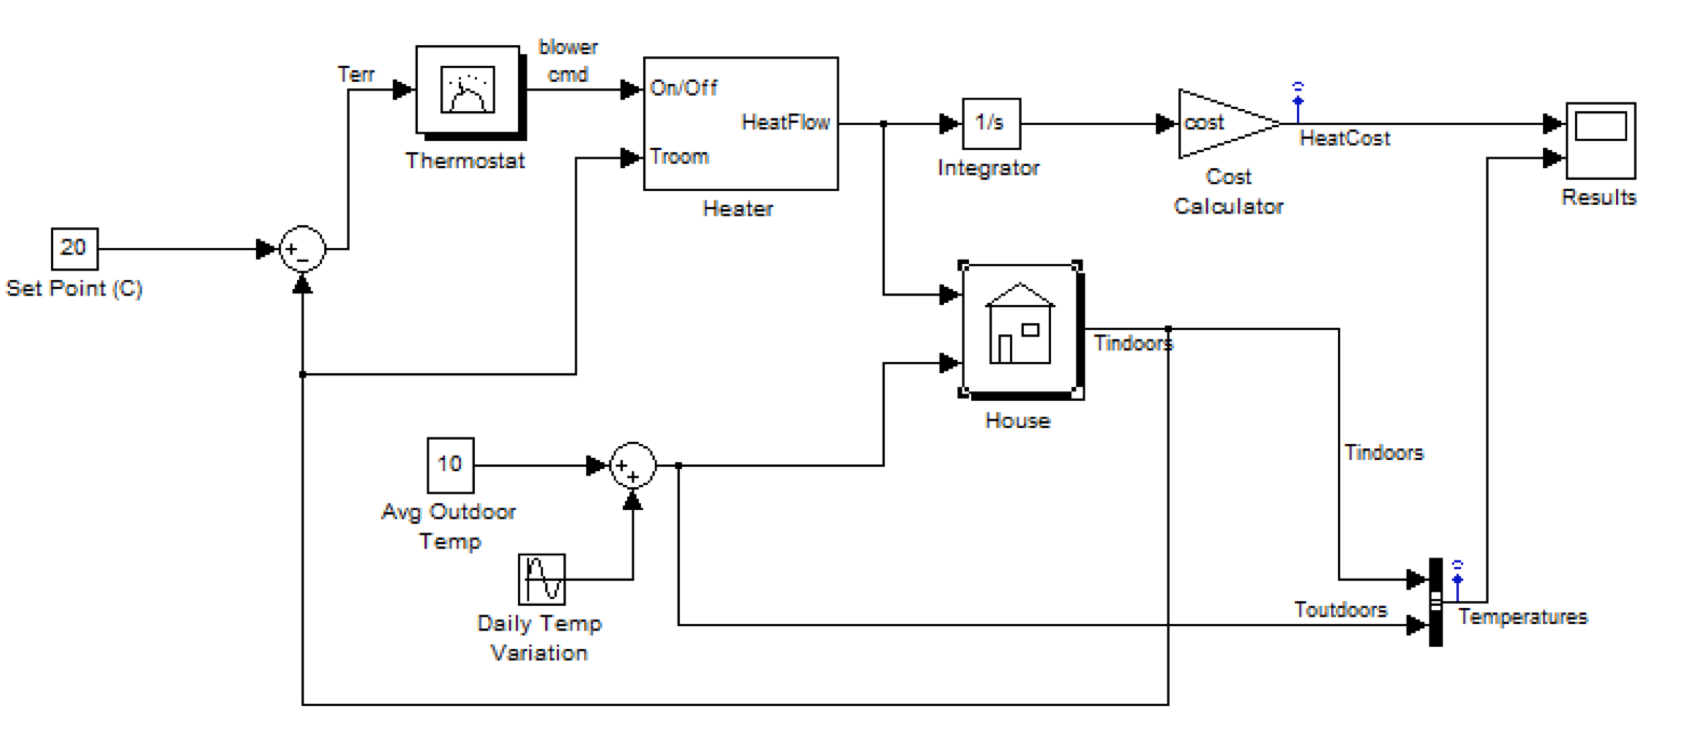
\includegraphics[width=1.0\linewidth]{1housetermo.png}
	\caption[Caption for LOF]{Original Simulink model with the binary thermostat.}
	\label{housetermo}
\end{figure}
The problem here is that the thermostat has only two states: On and Off. If the inside temperature differs significantly from the outside temperature, the thermostat starts up and heats the room until the ideal temperature of 18 C is reached. This leads to enormous oscillations in the inside temperature of the house, since the thermostat switches on and off continuously, especially at night when it cools down outside. This increases both energy consumption and heating costs. Figure \ref{origcost} shows the curves for the heating cost and the inside temperature:
\begin{figure}[H]
	\centering
	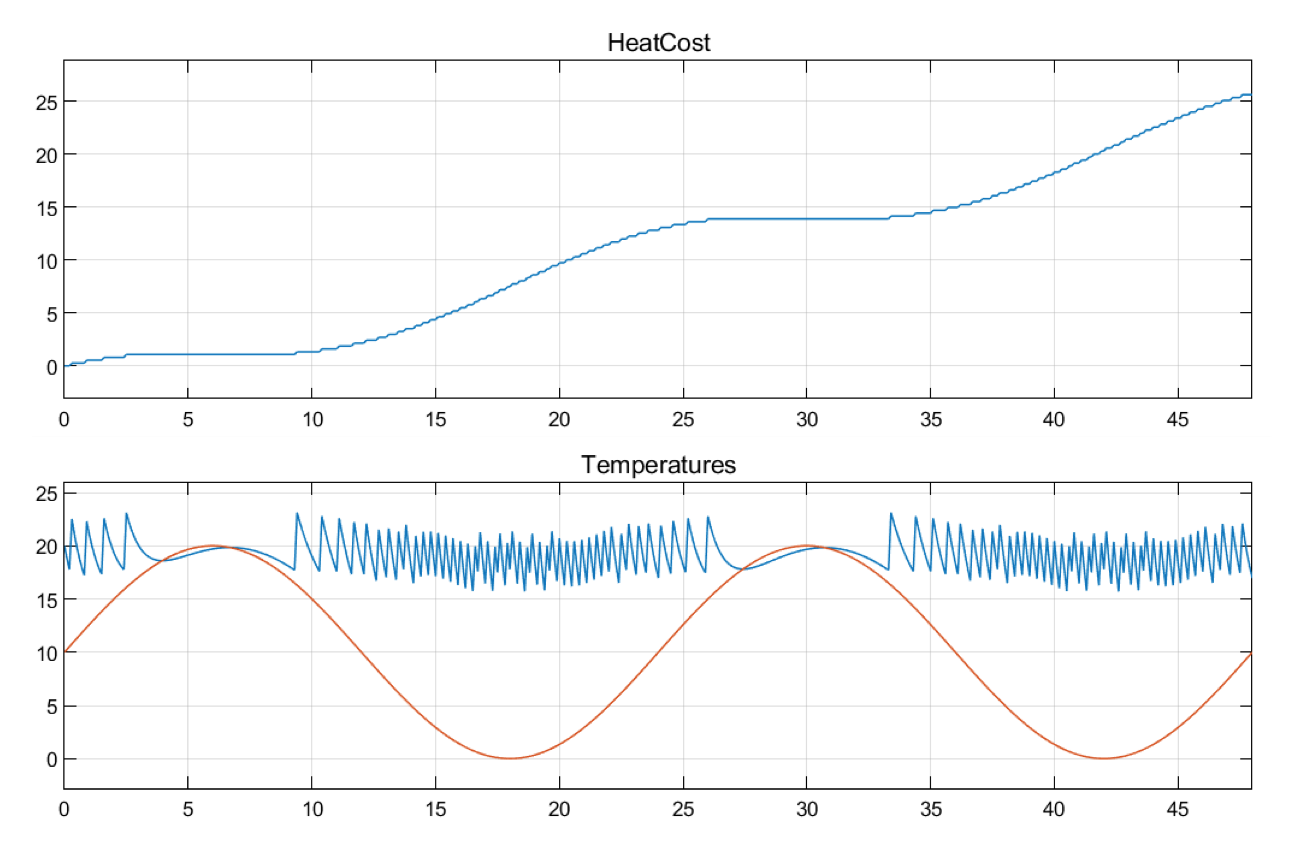
\includegraphics[width=1.0\linewidth]{1origcost.png}
	\caption[Caption for LOF]{Heat costs and temperatures( indoor: blue; outdoor: red) with the original binary setup.}
	\label{origcost}
\end{figure}
\section{The fuzzy controller}
The aim of the second part of the workshop is to replace the thermostat and its binary logic with a fuzzy controller that, instead of two states, has logic that allows the house model to control the strength of the heating system using percentages. 100\% or 1.0 represent the full power of the heating system and 0\% or 0.0 represent the OFF state.\\
Matlab allows, as with the ANN in part 1, to design a fuzzy logic controller that provides several inputs and outputs as well as the corresponding membership function and rulesets for configuration. In order to be able to implement the controller for the requirements described above, we need the outside temperature (\textit{outTem}p) as well as the deviation between outside and inside temperature (\textit{temperr}) as inputs. The output of the controller is the fan speed (\textit{fanSpeed}) of the heating system, which can be between 0.0 and 1.0. Figure \ref{fuzzycontroller} shows the setup for the fuzzy logic controller in Matlab:
\begin{figure}[H]
	\centering
	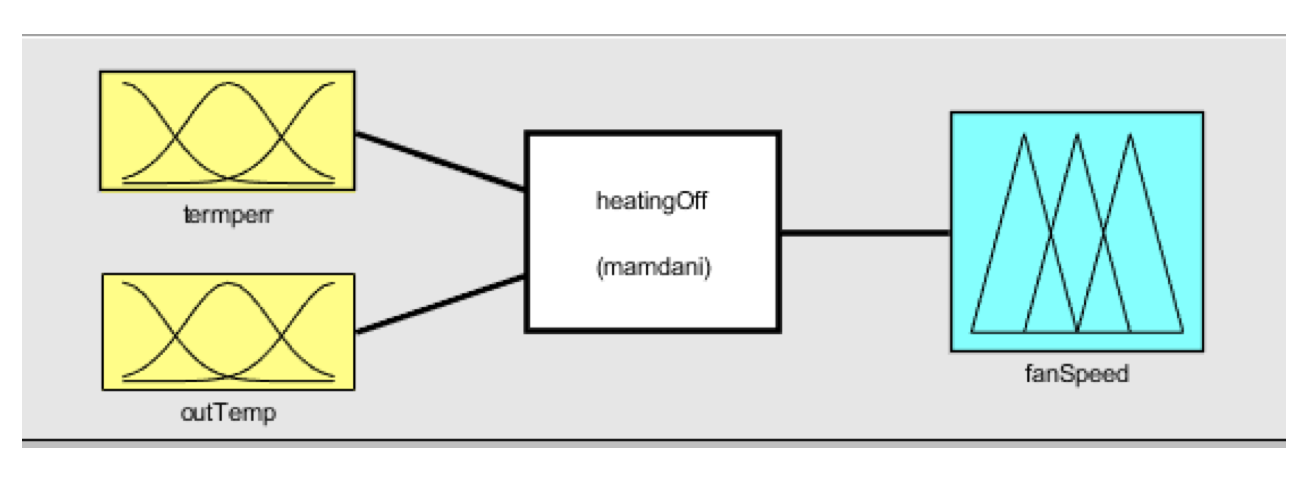
\includegraphics[width=1.0\linewidth]{1fuzzycontroller.png}
	\caption[Caption for LOF]{Fuzzy Logic Controller}
	\label{fuzzycontroller}
\end{figure}
The controller can be configured in Simulink with a fuzzy logic block. This then replaces the thermostat in the Simulink model of the house. The new setup can be seen in Figure \ref{housefuzzy}.
\begin{figure}[H]
	\centering
	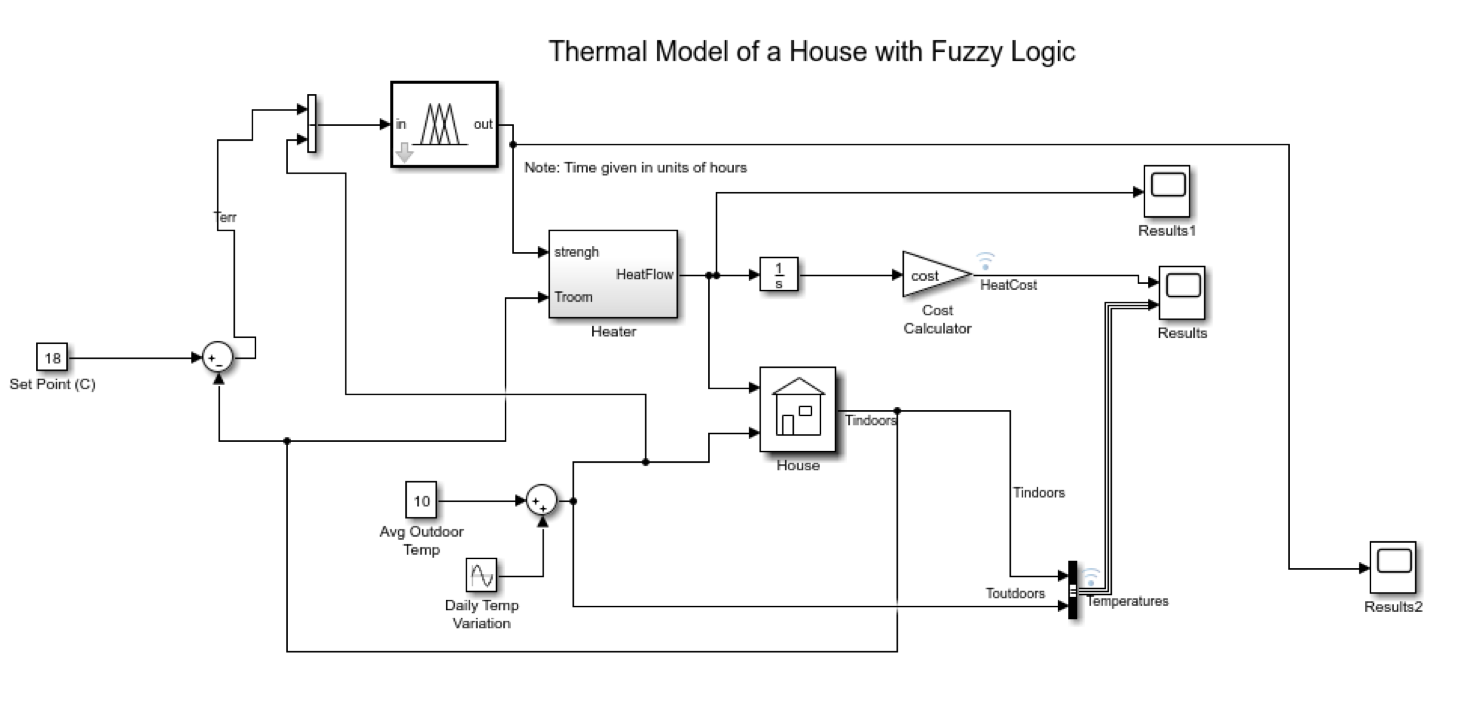
\includegraphics[width=1.0\linewidth]{1housefuzzy.png}
	\caption[Caption for LOF]{Modified Simulink model where the Fuzzy controller replaces the thermostat.}
	\label{housefuzzy}
\end{figure}
\subsection{Membership functions}
In order for the fuzzy controller to replace the thermostat and possibly provide better values, the correct membership function must be defined for both the inputs and the outputs. Based on these membership functions, a ruleset is then defined, which links the inputs with corresponding output values. Figure \ref{errorinput} shows the membership functions for the deviation between outside and inside temperature:
\begin{figure}[H]
	\centering
	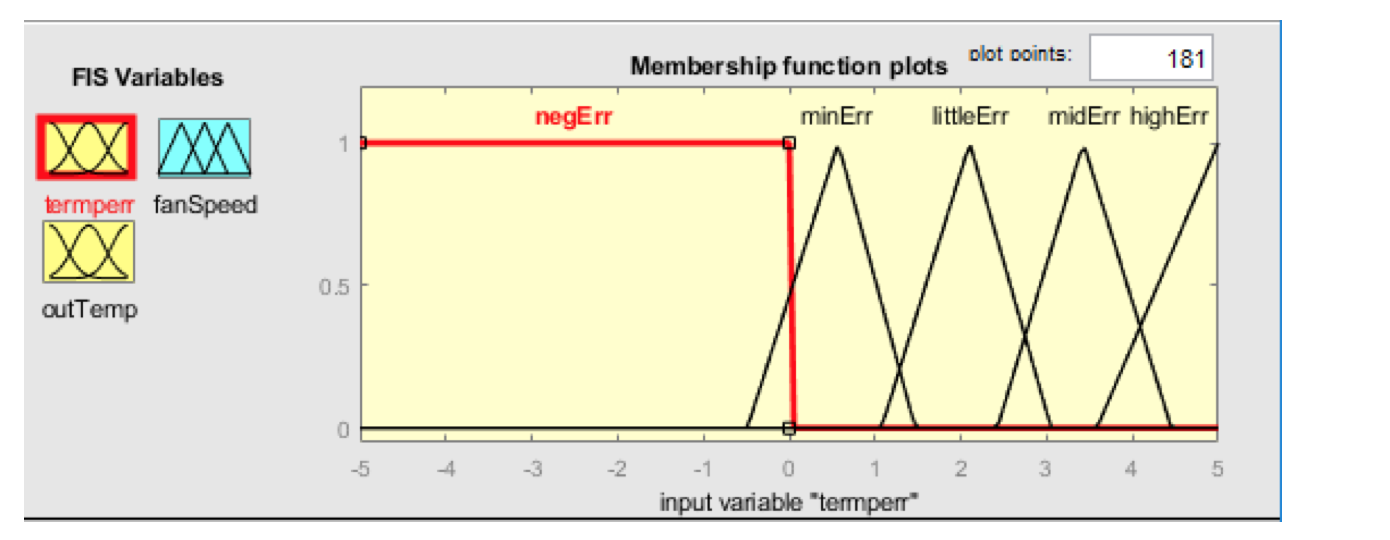
\includegraphics[width=1.0\linewidth]{1errorinput.png}
	\caption[Caption for LOF]{Membership function for temperature error.}
	\label{errorinput}
\end{figure}
The membership function for the Error defines multiple labels. the most important is the negError, which indicates that the outside temperature is already warmer than the inside temperature. It is extremely important that the heating system does not start up when it is warmer outside than indoors, as the temperature adjusts itself over time. The next figure shows the membership functions for the outside temperature:
\begin{figure}[H]
	\centering
	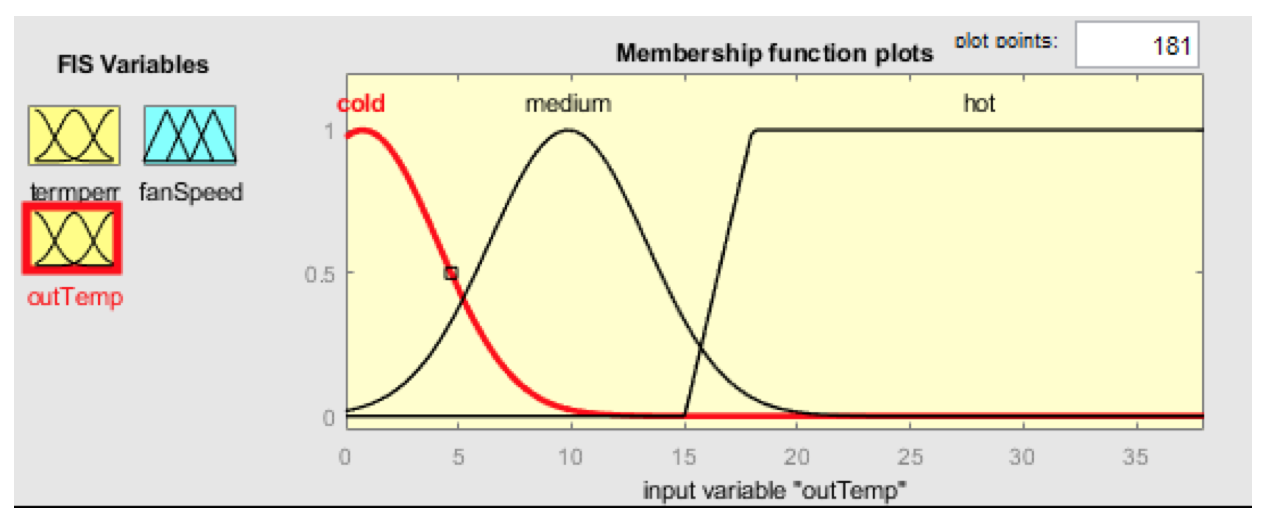
\includegraphics[width=1.0\linewidth]{1tempinput.png}
	\caption[Caption for LOF]{Membership function for the outdoor temperature.}
	\label{tempinput}
\end{figure}
It should be noted that all temperatures above 18 C are considered hot, which also ensures that the heating system does not start if the input values are in this range. The other functions for cold and medium follow Gaussian curves. The last figure shows the membership functions for the output values (\textit{fanSpeed}):
\begin{figure}[H]
	\centering
	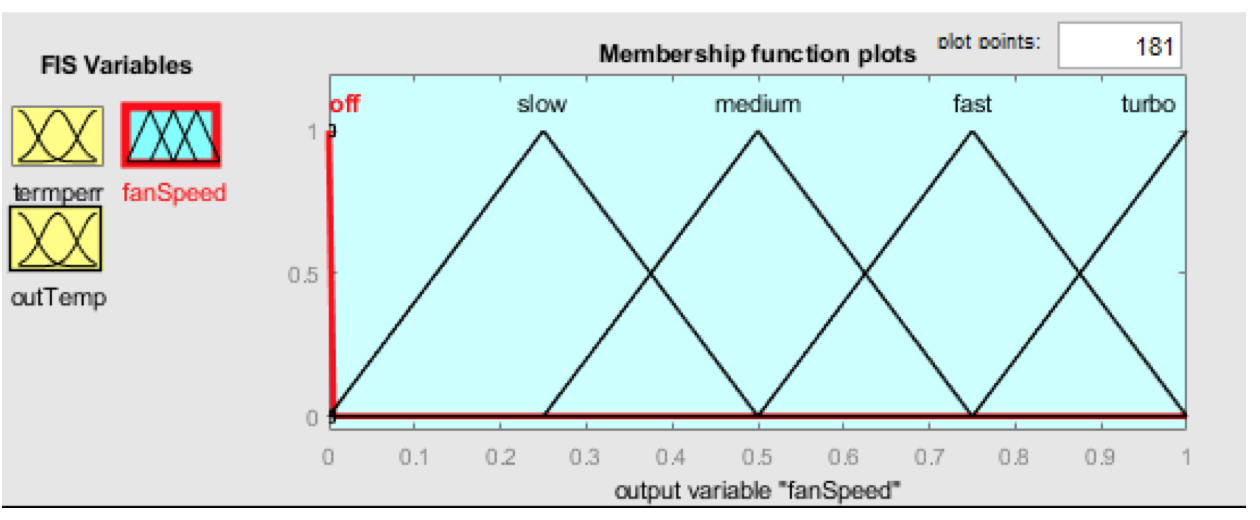
\includegraphics[width=1.0\linewidth]{1fanspeedoutput.png}
	\caption[Caption for LOF]{Membership function for the fanspeed of the heating system.}
	\label{fanspeedoutput}
\end{figure}
The functions overlap so that the values can be determined variably using fuzzy logic. Important here is the curve for Off. During the laboratory it was found that it is not smart that the curve for off in any way drives the heating system. Off should really be Off. Otherwise the system produces incorrect output values and the heating starts although the desired temperature has already been reached.
\subsection{Fuzzy Ruleset}
The last step to be taken for the fuzzy controller is to define a ruleset that maps the Input Membership Functions to the Output Membership functions and thus determines a value between 0.0 and 1.0 for the strength of the heating system. Figure \ref{fuzzyrules} shows the rule set for the Fuzzy Controller and thus the corresponding relations:
\begin{figure}[H]
	\centering
	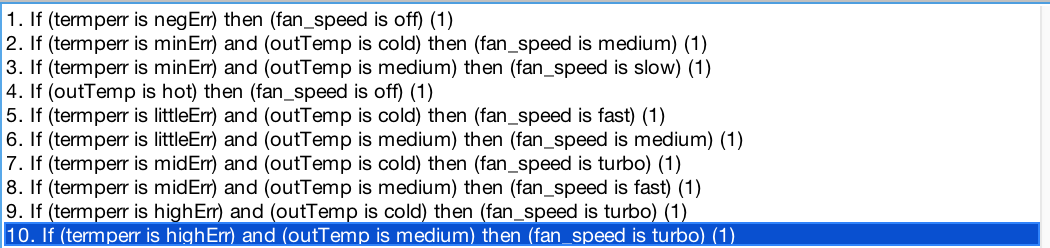
\includegraphics[width=1.0\linewidth]{1fuzzyrules.png}
	\caption[Caption for LOF]{Fuzzy rule set for controlling the fan speed.}
	\label{fuzzyrules}
\end{figure}
The most important rules here are that the Heater must not start if the error is negative or the outdoor temperature is already hot. The other rules are arranged according to logical contexts. The higher the error and the colder the outside temperature, the stronger the system must heat.
\section{Analysis and Evaluation}
After the new fuzzy controller was installed in the Simulink model and replaced the thermostat, the same measurement was made again for the indoor and outdoor temperature and for the cost calculation as in Chapter \ref{problem}. The following figure shows the results:
\begin{figure}[H]
	\centering
	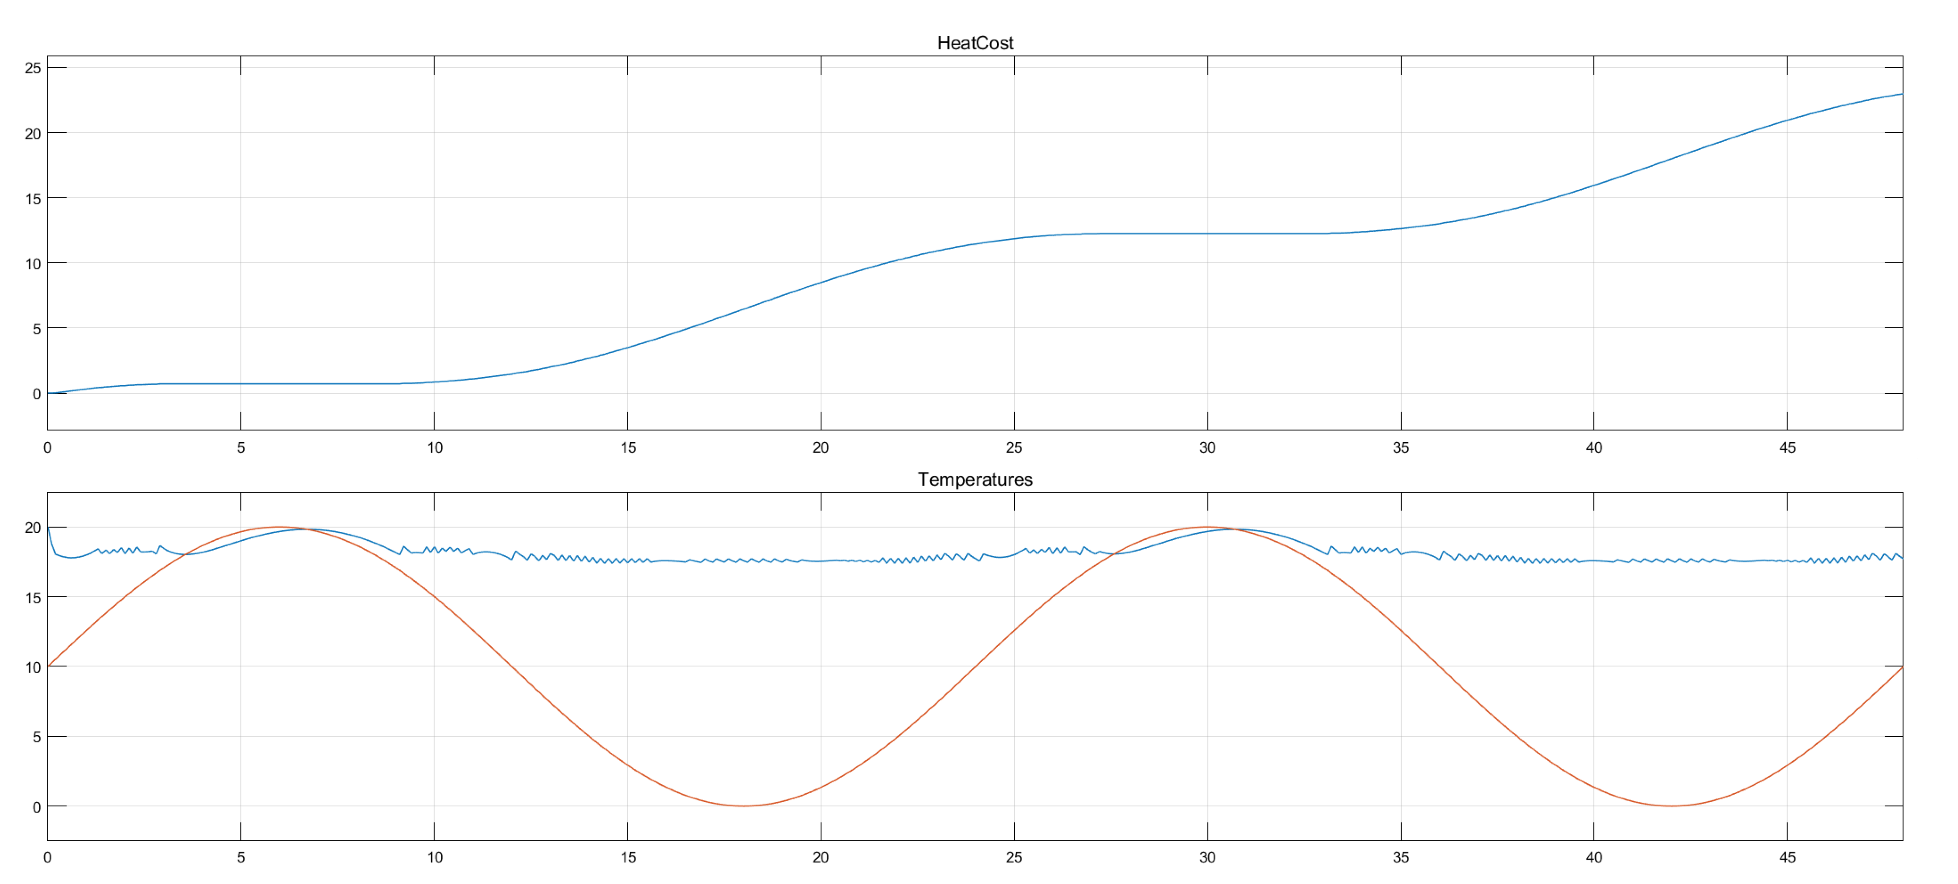
\includegraphics[width=1.0\linewidth]{1fuzzycost.png}
	\caption[Caption for LOF]{Heating costs and temperatures with fuzzy controller. Indoor (blue), outdoor (red).}
	\label{fuzzycost}
\end{figure}
As can be seen, the oscillations of the indoor temperature have decreased significantly and the curve is approaching the ideal value of 18 C. Only if the outdoor temperature exceeds the ideal value so will the indoor temperature rise with a slight delay. This is because the system can only heat and not cool. The costs for the heating system have also fallen in comparison. Even if the difference is not too big for one day, the energy savings add up over time. The following Figure \ref{energy} shows the heating over time:
\begin{figure}[H]
	\centering
	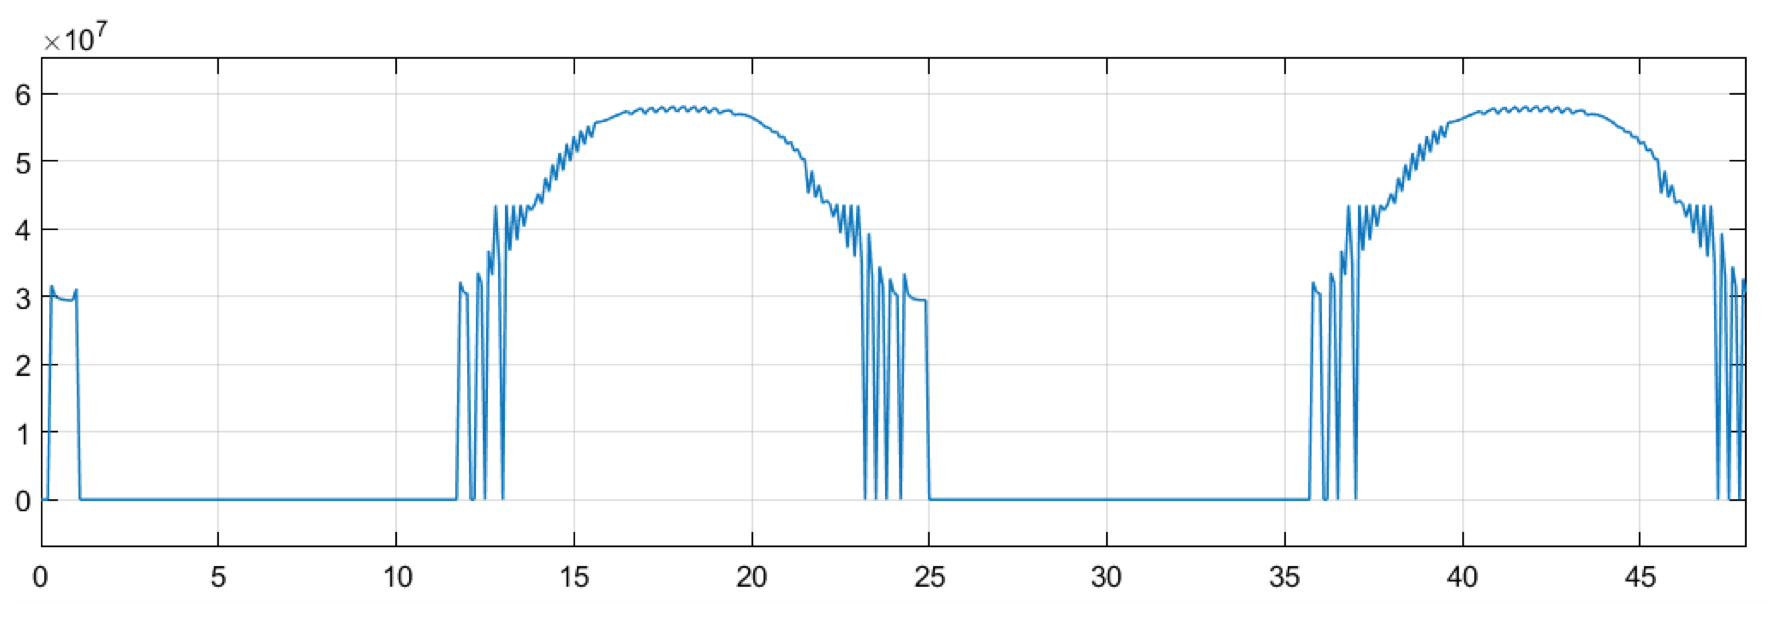
\includegraphics[width=1.0\linewidth]{1energy.png}
	\caption[Caption for LOF]{Heating Flow over time.}
	\label{energy}
\end{figure}
All in all, it can be seen that the system can be implemented much more precisely and energy-saving if a fuzzy controller is used instead of a thermostat with binary logic.
%%%%%%%%%%%%%%%%%%%%%%%%%%%%%%%%%%%%%%%%%%%%%%%%%%%%%%%%%%%%%%%%%%%%%%%%%%%%%%%%%%%%%%%%%%%%%%%%%%%%%%%%%
%%%%%%%%%%%%%%%%%%%%%%%%%%%%%%%%%%%%%%%%%%%%%%%%%%%%%%%%%%%%%%%%%%%%%%%%%%%%%%%%%%%%%%%%%%%%%%%%%%%%%%%%%
%%%%%%%%%%%%%%%%%%%%%%%%%%%%%%%%%%%%%%%%%%%%%%%%%%%%%%%%%%%%%%%%%%%%%%%%%%%%%%%%%%%%%%%%%%%%%%%%%%%%%%%%%
\chapter{Conclusion}
\label{conlusion}
This assignment has shown how easily intelligent machine learning technologies can replace complex logic and functionalities. This became particularly clear when the house model was replaced by the Artificial Neural Network in part 1 of the workshop and the results came very close. All it took was reliable training data.\\
The second part on fuzzy logic, on the other hand, dealt with the more precise decision-making of intelligent systems. For a long time computers have not been able to make more complicated decisions like humans for more complex situations. Computers usually only knew binary patterns. Either a statement was true or false. There was nothing in between. This problem can be solved with Fuzzy Logic, as we saw in the second part of the assignment. All that is needed are correctly defined rule sets and membership functions for the inputs and outputs of a fuzzy controller. 
\\Matlab and Simulink make it easy for a developer here, as they already offer the corresponding functions for both ANNs and fuzzy logic.


